\documentclass[aspectratio=43,english]{beamer} %If you want to create Polish presentation, replace 'english' with 'polish' and uncomment 3-th line, i.e., '\usepackage{polski}'
\usepackage[utf8]{inputenc}
\usepackage{polski} %Uncomment for Polish language
\usepackage{babel}
\usepackage{listings} %We want to put listings

\mode<beamer>{ 	%in 'beamer' mode
	\hypersetup{pdfpagemode=FullScreen}		%Enable Full screen mode
	\usetheme{JuanLesPins} 		%Show part title in right footer
	%\usetheme[dark]{AGH}                 		%Use dark background
	%\usetheme[dark,parttitle=leftfooter]{AGH}  	%Use dark background and show part title in left footer
}
\mode<handout>{	%in 'handout' mode
	\hypersetup{pdfpagemode=None}		
	\usepackage{pgfpages}
  	\pgfpagesuselayout{4 on 1}[a4paper,border shrink=5mm,landscape]	%show 4 slides on 1 page
  	\usetheme{boxes}
  	\addheadbox{structure}{\quad\insertpart\hfill\insertsection\hfill\insertsubsection\qquad} 	%content of header
 	\addfootbox{structure}{\quad\insertauthor\hfill\insertframenumber\hfill\insertsubtitle\qquad} 	%content of footer
}

\AtBeginPart{ %At begin part: display its name
	\frame{\partpage}
} 


%%%%%%%%%%% Configuration of the listings package %%%%%%%%%%%%%%%%%%%%%%%%%%
% Source: https://en.wikibooks.org/wiki/LaTeX/Source_Code_Listings#Using_the_listings_package
%%%%%%%%%%%%%%%%%%%%%%%%%%%%%%%%%%%%%%%%%%%%%%%%%%%%%%%%%%%%%%%%%%%%%%%%%%%%
\lstset{ %
  backgroundcolor=\color{white},   % choose the background color
  basicstyle=\footnotesize,        % the size of the fonts that are used for the code
  breakatwhitespace=false,         % sets if automatic breaks should only happen at whitespace
  breaklines=true,                 % sets automatic line breaking
  captionpos=b,                    % sets the caption-position to bottom
  commentstyle=\color{green},      % comment style
  deletekeywords={...},            % if you want to delete keywords from the given language
  escapeinside={\%*}{*)},          % if you want to add LaTeX within your code
  extendedchars=true,              % lets you use non-ASCII characters; for 8-bits encodings only, does not work with UTF-8
  frame=single,	                   % adds a frame around the code
  keepspaces=true,                 % keeps spaces in text, useful for keeping indentation of code (possibly needs columns=flexible)
  keywordstyle=\color{blue},       % keyword style
  morekeywords={*,...},            % if you want to add more keywords to the set
  numbers=left,                    % where to put the line-numbers; possible values are (none, left, right)
  numbersep=5pt,                   % how far the line-numbers are from the code
  numberstyle=\tiny\color{gray},   % the style that is used for the line-numbers
  rulecolor=\color{black},         % if not set, the frame-color may be changed on line-breaks within not-black text (e.g. comments (green here))
  showspaces=false,                % show spaces everywhere adding particular underscores; it overrides 'showstringspaces'
  showstringspaces=false,          % underline spaces within strings only
  showtabs=false,                  % show tabs within strings adding particular underscores
  stepnumber=2,                    % the step between two line-numbers. If it's 1, each line will be numbered
  stringstyle=\color{cyan},        % string literal style
  tabsize=2,	                   % sets default tabsize to 2 spaces
  title=\lstname,                  % show the filename of files included with \lstinputlisting; also try caption instead of title
                                   % needed if you want to use UTF-8 Polish chars
  literate={?}{{\k{a}}}1
           {?}{{\k{A}}}1
           {?}{{\k{e}}}1
           {?}{{\k{E}}}1
           {�}{{\'o}}1
           {�}{{\'O}}1
           {?}{{\'s}}1
           {?}{{\'S}}1
           {?}{{\l{}}}1
           {?}{{\L{}}}1
           {?}{{\.z}}1
           {?}{{\.Z}}1
           {?}{{\'z}}1
           {?}{{\'Z}}1
           {?}{{\'c}}1
           {?}{{\'C}}1
           {?}{{\'n}}1
           {?}{{\'N}}1
}
%%%%%%%%%%%%%%%%%


\title{Metody Obliczeniowe w Nauce i Technice}
\author{Marian Bubak, PhD}
\date{}
\institute[AGH]{
	Institute of Computer Science\\ul. Kawiory 21\\30-055 Krakow\\
	Poland\\
	\url{http://www.icsr.agh.edu.pl/~mownit/}
}



\subtitle{8. Wyznaczanie pierwiastków wielomianów}
\setcontributors{Magdalena Nowak\\Paweł Taborowski\\Arkadiusz Placha}


\begin{document}
  \maketitle
	\begin{frame}{Plan wykładu}
		\tableofcontents
	\end{frame}

  \section{Wstęp}

\begin{frame}{Wstęp}
  \begin{block}{}
    $$ f(x) = \sum_{i=0}^m a_i \cdot x^i = 0; \qquad a_m \neq 0 $$
  \end{block}

  \begin{itemize}
    \item Wielomian stopnia $m$ -- $m$ pierwiastków,
    \item Jeżeli $a_i$ -- rzeczywiste, to ewentualne pierwiastki zespolone są parami sprzężone:
    $$ \alpha + \textit{\textrm{i}} \cdot \beta, \quad \alpha - \textit{\textrm{i}} \cdot \beta $$
    \item Jeżeli $a_i$ -- zespolone, to brak związku między pierwiastkami.
  \end{itemize}
\end{frame}

\begin{frame}
  Szukanie zer -- dobór metody:
  \begin{itemize}
    \item Dowolny
    \item Ze względu na postać $f(x)$ -- metody specjalne (zwłaszcza dla w. zespolonych).
  \end{itemize}

  Trudności:
  \begin{itemize}
    \item Wielokrotne pierwiastki -- trudno ,,obramować'', łatwiej, gdy znana krotność,
    \item Blisko położone pierwiastki -- trudności jak wyżej.
  \end{itemize}

  \textit{Nie wiadomo z góry, jaki typ patologii wykazuje wielomian.}

  \vspace{5px}

  \begin{alertblock}{Uwaga}
      \textit{Zadanie wyznaczania zer wielomianów może być źle uwarunkowane.} (Wilkinson).
  \end{alertblock}
  % Wilkinson: rozwinąć temat
\end{frame}

\begin{frame}
  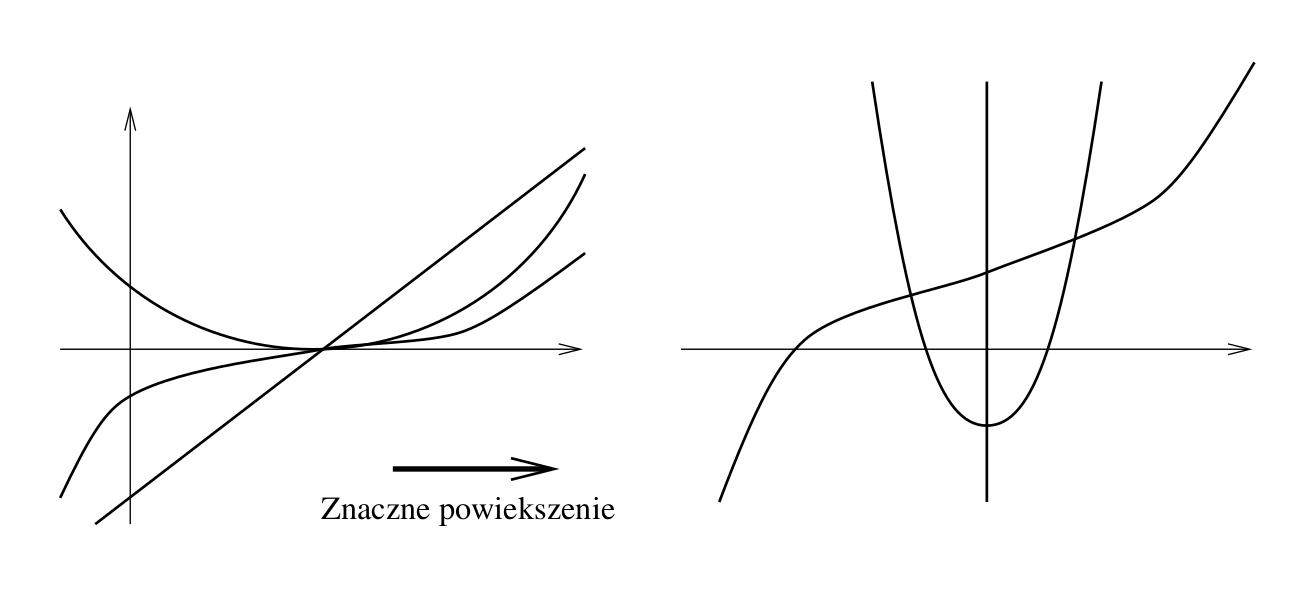
\includegraphics[width=\textwidth]{img/8/wielomian}
\end{frame}


  \section{Deflacja -- dzielenie syntetyczne}

\begin{frame}{Deflacja -- dzielenie syntetyczne}
  \textbf{Deflacja} -- bardzo użyteczny element wyznaczania pierwiastków wielomianów. % Deflacja – obniżenie stopnia wielomianu po znalezieniu jego pierwiastka; bardzo użyteczna część algorytmu wyznaczania pierwiastków wielomianów.

  \begin{block}{Nested form (Horner)}
    $$ f(x) = \sum_{i=0}^m a_i \cdot x^i = ( ( \dots (( a_m \cdot x + a_{m-1}) \cdot x + a_{m-2} ) \cdot \dots) \cdot x + a_1) \cdot x + a_0 $$
  \end{block}
\end{frame}

\begin{frame}
  Rekurencyjny algorytm obliczania wartości wielomianu dla $x = \lambda$ ma postać:

  \begin{block}{Algorytm}
    $$ \left \{ \begin{array}{l}
    b_{m-1} = a_m \\
    b_i = a_{i+1} + \lambda \cdot b_{i+1}, \quad i = m - 2, m-3, \dots, 0 \\
    f( \lambda ) = a_{0} + \lambda \cdot b_{0}
    \end{array} \right. $$
  \end{block}
\end{frame}

\begin{frame}

  \begin{block}{Twierdzenie}
    $$ \frac{f(x) - f(\lambda)}{x - \lambda} = \sum_{i=0}^{m-1} b_i x^i $$
  \end{block}

  Dowód:

  \begin{itemize}
    \item mnożenie przez $(x - \lambda)$
    \item $ b_{i-1} = a_i + \lambda \cdot b_i $
  \end{itemize}

  \vspace{5px}

  \textbf{Zadanie:} Przeprowadzić dowód.
\end{frame}


  \subsection{Deflacja czynnikiem liniowym}

\begin{frame}{Deflacja czynnikiem liniowym}
  \begin{block}{}
    $$ f(x) = (x - \lambda) \cdot \underbrace{\sum_{i=0}^{m-1} b_i x^i}_{g(x)} + f(\lambda) \qquad (*) $$
  \end{block}
  gdy $ \lambda = \alpha $, wtedy $x$: pierwiastek $ f(x) = 0 $

  \vspace{5px}

  pozostałe zera $f(x) = 0$: $ g(x) = \sum_{i=0}^{m-1} b_i x^i $ \qquad deflated equation

  \vspace{5px}

  \begin{alertblock}{Uwaga}
    Ale następuje kumulowanie błędów: $\alpha$ z błędem, $b_i$ z błędem itd\dots
  \end{alertblock}
\end{frame}

\begin{frame}
  \textbf{Pochodna} -- Różniczkując równanie (*)

  $$ f'(x) = (x - \lambda) \cdot g'(x) + g(x) $$
  $$ f'(x) = g(\lambda) $$
\end{frame}


  \subsection{Deflacja czynnikiem kwadratowym: $ x^2 +px + q $}

\begin{frame}{Deflacja czynnikiem kwadratowym: $ x^2 +px + q $}
  \begin{block}{}
    $$ f(x) \equiv \sum_{i=0}^m a_i x^i \equiv (x^2 + px + q) \cdot \sum_{i=0}^{m-2} c_i x^i + Rx +S $$
  \end{block}

  \vspace{6mm}

  Przez porównanie współczynników:

  $$ \left \{ \begin{array}{l}
  c_{m-2} = a_m \\
  c_{m-3} = a_{m-1} - p \cdot c_{m-2} \\
  c_i = a_{i+2} - p \cdot c_{i+1} - q \cdot c_i + 2, \qquad i = m - 4, m - 5, \dots , 0 \\ % +2 NIEMAL NA PEWNO POWINNO BYĆ W INDEKSIE DOLNYM
  R = a_1 - p \cdot c_0 - q \cdot c_1 \\
  S = a_0 - q \cdot c_0
  \end{array} \right. $$
\end{frame}

\begin{frame}
  Można to zapisać wygodniej, przyjmując $ c_m = c_{m-1} = 0 $, $ c_{-1} = R $:

  \begin{block}{}
    $$ \left \{ \begin{array}{l}
    c_i = a_{i+2} - p \cdot c_{i+1} - q \cdot c_i + 2, \qquad i = m-2, m-3, \dots , 0, -1 \\
    S = a_0 - q \cdot c_0
    \end{array} \right. $$
  \end{block}

  \textbf{Zadanie:} Sprawdzić.

  \vspace{5px}

  Oczywiście: $ c_i = c_i(p,q), R = R(p,q), S = S(p,q) $

  \vspace{5px}

  Jeżeli $p,q$ takie, że $R(p,q) = 0$ i $S(p,q) = 0$ to \\ $x^2 + px + q$ -- czynnik kwadratowy $f(x)$, \\i z niego dwa pierwiastki $f(x)$ (ewentualnie zespolone).
\end{frame}


  \subsection{Przydatność deflacji}

\begin{frame}{Przydatność deflacji}
  $P(x)$ -- wielomian,

  $r$ -- znaleziony pierwiastek wielomianu $P$.

  Realizujemy \textit{faktoryzację}:
  \begin{block}{}
    $$ P(x) = (x - r) \cdot Q(x) $$
  \end{block}

  \begin{itemize}
    \item Zmniejszenie złożoności obliczeniowej\\
     ($Q$ -- niższego stopnia niż $P$)
    \item Uniknięcie pomyłki -- powrotu do pierwiastka już znalezionego.
  \end{itemize}
\end{frame}

\begin{frame}
  Stosowanie deflacji musi być \textbf{ostrożne!}

  \textbf{Powód:} -- pierwiastki są wyznaczane ze skończoną dokładnością (kilka deflacji pociąga kumulację błędu).

  \begin{block}{}
    \begin{itemize}
      \item \textbf{Forward deflation} -- nowe współczynniki $Q(x)$ obliczane od najwyższych potęg $x$ \dots Stabilna, gdy zaczynamy od pierwiastków o \textbf{najmniejszej} wartości bezwzględnej,
      \item \textbf{Backward deflation} -- współczynniki $Q(x)$ wyznaczane poczynając od wyrazu wolnego \dots Stabilna, gdy zaczynamy od pierwiastków o \textbf{największej} wartości bezwzględnej.
    \end{itemize}
  \end{block}

  \textbf{Zadanie:} Dlaczego?
\end{frame}

\begin{frame}
  \begin{block}{Podejście minimalizujące błędy}
    \begin{itemize}
      \item Kolejne pierwiastki uzyskane w procesie deflacji są \textit{próbnymi (tentative)},
      \item \textit{Polishing (re-solving)} -- wygładzanie -- z użyciem pełnego $P(x)$ np. metodą Newtona-Raphsona,
      \item Niebezpieczeństwo -- zlanie się dwóch pierwiastków w jeden.\\
        Dodatkowa deflacja tylko jeden raz.
    \end{itemize}
  \end{block}
\end{frame}


  \section{Metoda Laguerre'a znajdowania pierwiastków wielomianu}

\begin{frame}{Met. Laguerre'a znajdowania pierwiastków wielomianu}
  \begin{block}{Metoda ogólna}
    \begin{itemize}
      \item dla pierwiastków rzeczywistych i zespolonych,
      \item dla pierwiastków pojedynczych i wielokrotnych,
      \item \textit{most straightforward},
      \item \textit{sure-fire}.
    \end{itemize}
  \end{block}
\end{frame}

\begin{frame}
  \textbf{Istota} wynika z poniższych związków między:
  \begin{itemize}
    \item wielomianem,
    \item jego pierwiastkami,
    \item jego pochodnymi:
  \end{itemize}

  \begin{block}{}
    $$ \begin{array}{ll}
    (1) & P_n(x) = (x - x_1) \cdot (x - x_2) \cdot \ldots \cdot (x - x_n) \\
    (2) & \ln|P_n(x)| = \ln|x - x_1| + \ln|x - x_2| + \ldots + \ln|x - x_n| \\
    (3) & \frac{d \ln|P_n(x)|}{dx} = \frac{1}{x - x_1} + \frac{1}{x - x_2} + \ldots + \frac{1}{x - x_n} = \frac{P'_n(x)}{P_n(x)} \equiv G \\
    (4) & -\frac{d^2 \ln|P_n(x)|}{dx^2} = \frac{1}{(x - x_1)^2} + \frac{1}{(x - x_2)^2} + \ldots + \frac{1}{(x - x_n)^2} = \\
    & = \left[ \frac{P'_n(x)}{P_n(x)} \right] ^2 - \frac{P''_n(x)}{P_n(x)} \equiv H
    \end{array} $$
  \end{block}
\end{frame}

\begin{frame}
  W oparciu o te związki -- drastyczne założenie:
  \begin{block}{Założenie}
    \begin{tabular}{ll}
      $x$ & odgadnięte (bieżące) położenie \\
      & pierwiastka \\
      $a = x - x_1$ & odległość od pierwiastka \\
      $b = x - x_i, i = 2,3, \dots , n$ & odległość pozostałych pierwiastków
    \end{tabular}
  \end{block}

  \begin{block}{Wniosek}
    $$ \left. \begin{array}{rcl}
      \text{wtedy z } (3) & : & \frac{1}{a} + \frac{m+1}{b} = G \\ % Czymkolwiek nie byłoby m; Wikipedia proponuje n-1, gdzie n – stopień wielomianu
      (4) & : & \frac{1}{a^2} + \frac{m+1}{b^2} = H
    \end{array} \right\} $$
  \end{block}

$G$, $H$ -- wyznaczone dla aktualnego $x$ (z $P$, $P'$, $P''$!!!)
\end{frame}

\begin{frame}
  \begin{block}{rozwiązanie układu}
    $$a = \frac{n}{G \pm \sqrt{(n-1)(nH-G^2)}}$$
  \end{block}

  \textbf{Zadanie:} Sprawdzić

  \begin{itemize}
    \item bierzemy rozwiązanie dające mniejsze $a$,
    \item $a$ może być zespolone $\Rightarrow$ metoda ,,sama z siebie'' zaczyna przeszukiwać $z$, % O jakie z chodzi? – Prawdopodobnie o Z tudzież C – zbiór liczb zespolonych
    \item rozpoczynamy od przybliżenia $x$, potem $(x-a),\dots $
  \end{itemize}
\end{frame}

\begin{frame}
  \begin{block}{}
    \begin{description}
      \item[Zaleta:] dla $P(x)$ o współczynnikach rzeczywistych -- zbieżna niezależnie od wyboru początkowego $x$.
      \item[Wada:] potrzebne $P$, $P'$, $P''$ w każdym kroku.
    \end{description}
  \end{block}

  Więcej o metodzie -- przykłady konkretnych rozwiązań \cite{Adams}
\end{frame}


  \section{Techniki wygładzania pierwiastków (root polishing)}

  \subsection{Pierwiastki rzeczywiste -- metoda Newtona-Raphsona}

\begin{frame}{Techniki wygładzania pierwiastków (root polishing) \\Pierwiastki rzeczywiste -- metoda Newtona-Raphsona}
  \begin{itemize}
    \item wielomian stopnia $N-1$,
    \item współczynniki: $C(1), C(2), \dots, C(N)$; $C(N)$ -- przy $x^{N-1}$
  \end{itemize}

  $$\begin{array}{ll}
  P = C(N) \cdot x + C(N-1) & \rightarrow P(x) \\
  P_1 = C(N) & \rightarrow P'(x)
  \end{array}$$
\end{frame}

\begin{frame}[fragile]
  % Kod niepoprawny
  \begin{lstlisting}[language=Pascal]
do 1 i = N-2,1,-1
  P = C(i) + P%*$\cdot$*)x
  P = P + P%*$_1\cdot$*)x
1 continue
  if (P%*$_1\cdot$*)eq.  0.0)%*$\Rightarrow$*)alarm
X = X-P/P%*$_1$*)
\end{lstlisting}

  \textbf{Zadanie:} sprawdzić poprawność
\end{frame}


  \subsection{Pierwiastki zespolone -- metoda Bairstowa}

\begin{frame}{Pierwiastki zespolone -- metoda Bairstowa}
  \textit{(można też metodą N-R)}

  \vspace{5px}

  \textbf{Metoda Bairstowa} polega na szukaniu czynników kwadratowych

  $$x_1 = \alpha + \textit{\textrm{i}}\beta, \quad x_2 = \alpha - \textit{\textrm{i}}\beta$$
  $$(x - x_1)(x - x_2) = x^2 - 2 \cdot \alpha x + (\alpha^2 + \beta^2) = x^2 + p \cdot x + q$$

  czynnik kwadratowy może objąć 2 pierwiastki rzeczywiste lub zespolone

  \begin{equation}
    P(x) = (x^2 + p \cdot x + q) \cdot Q(x) + R \cdot x + S \label{bairstow}
  \end{equation}
\end{frame}

\begin{frame}
  $$\left. \begin{array}{l}
  R(p,q)=0 \\ S(p,q)=0
  \end{array}\right\} \Rightarrow \text{met. Newtona-Raphsona}$$

  \vspace{5mm}

  $$\left( \begin{array}{l}
  p^{(n+1)} \\ q^{(n+1)}
  \end{array} \right)
  =
  \left( \begin{array}{l}
  p^{(n)} \\ q^{(n)}
  \end{array} \right)
  +
  \left( \begin{array}{ll}
  \frac{{\partial}R}{{\partial}p} & \frac{{\partial}R}{{\partial}q} \\
  \frac{{\partial}S}{{\partial}p} & \frac{{\partial}S}{{\partial}q}
  \end{array} \right)_n^{-1}
  \left( \begin{array}{l}
  R^{(n)} \\ S^{(n)}
  \end{array} \right)$$
\end{frame}

\begin{frame}
  Pochodne znajdujemy w następujący sposób:

  $P(x)$ -- nie zależy od $p$, $q$, \\ z (\ref{bairstow}) mamy:

  $$\left. \begin{array}{l}
  0 = (x^2 + p \cdot x + q) \cdot \frac{{\partial}Q}{{\partial}q} + Q + \frac{{\partial}R}{{\partial}q} + \frac{{\partial}S}{{\partial}q} \\ % NIE POWINNO BYĆ *x PRZY R'???
  0 = (x^2 + p \cdot x + q) \cdot \frac{{\partial}Q}{{\partial}p} + x \cdot Q + \frac{{\partial}R}{{\partial}p} + \frac{{\partial}S}{{\partial}p} % NIE POWINNO BYĆ *x PRZY R'???
  \end{array}\right\}
  \begin{array}{l}
    \left( \leftarrow \frac{{\partial}R}{{\partial}q} \right) \\
    \left( \leftarrow \frac{{\partial}R}{{\partial}q} \right) % NAPRAWDĘ NIE POWINNO BYĆ PO p?
  \end{array}$$

  \begin{equation}
    \left. \begin{array}{l}
    (x^2 + p \cdot x + q) + \frac{{\partial}Q}{{\partial}q} + \frac{{\partial}R}{{\partial}q} \cdot x + \frac{{\partial}S}{{\partial}q} = -Q(x) \\ % NIE POWINNO BYĆ * dQ/dq ??? (zamiast +)
    (x^2 + p \cdot x + q) + \frac{{\partial}Q}{{\partial}p} + \frac{{\partial}R}{{\partial}p} \cdot x + \frac{{\partial}S}{{\partial}p} = -x \cdot Q(x) % NIE POWINNO BYĆ * dQ/dp ??? (zamiast +)
    \end{array}\right\}
    \label{bairstow2}
  \end{equation}
\end{frame}

\begin{frame}
  (\ref{bairstow2}) mają podobną strukturę jak (\ref{bairstow}) $\rightarrow$ pochodne $\frac{{\partial}R}{{\partial}p}$, $\frac{{\partial}R}{{\partial}q}$, $\frac{{\partial}S}{{\partial}p}$, $\frac{{\partial}S}{{\partial}q}$ \\ \vspace{2mm} mogą być uzyskane przez syntetyczne dzielenie wielomianów \\ \vspace{3mm} $\left.\begin{array}{l} -Q(x) \\ -x Q(x) \end{array} \right\}$ przez czynnik kwadratowy.
\end{frame}


  \subsection{Metoda Maehly'ego -- technika wygładzania pierwiastków}

\begin{frame}{Met. Maehly'ego -- technika wygładzania pierwiastków}
  Zapobiega zlewaniu się w jeden dwóch różnych pierwiastków (na~etapie wygładzania) $\leftarrow$ równocześnie unikamy deflacji.

  \begin{block}{Zredukowany wielomian}
    $$P_j(x) \equiv \frac{P(x)}{(x - x_1)\ldots(x - x_j)}$$
  \end{block}
  
  $$P'_j(x) = \frac{P'(x)}{(x - x_1)\ldots(x - x_j)} - \frac{P(x)}{(x - x_1)\ldots(x - x_j)} \sum_{i/1}^j \frac{1}{x - x_i}$$ % CZEMU "i/1"?? NIE MOŻNA "="??
\end{frame}

\begin{frame}
  Pojedynczy krok metody Newtona-Raphsona można zapisać:

  $$x_{k+1} = x_k - \frac{P_j(x_k)}{P'_j(x_k)}$$

  czyli:

  $$x_{k+1} = x_k - \frac{P(x_k)}{P'(x_k) - P(x_k) \cdot \sum_{j/0}^j(x - x_i)^{-1}}$$ % INDEKS JEST NA PEWNO ZŁY.

  \textbf{Zadanie:} i- po węzłach już wygładzonych % NIE MAM POJĘCIA, O CO CHODZI, CZEGOŚ TU BRAKUJE...

  $\Rightarrow$ zero suppression.
\end{frame}


  \section{Bibliografia}

  \begin{frame}{Bibliografia}
      \begin{thebibliography}{9}
          \setbeamertemplate{bibliography item}[article]
              \bibitem[ADAMS]{Adams}{Adams, Arthur G. \newblock Remark on Algorithm 304 [S15]: Normal Curve Integral \newblock Commun. ACM, 1969}
      \end{thebibliography}
  \end{frame}

\end{document}
